\documentclass{article}
\usepackage{amsmath,amssymb}
\usepackage{bm}
\usepackage{multirow}
\usepackage{dcolumn}
\usepackage{verbatim}
%\topmargin=0cm
%\textheight=650pt
%\headsep=0pt
%\headheight=0pt
\textheight650pt
\textwidth470pt

\marginparwidth0pt
\marginparsep0pt
\marginparpush0pt
\evensidemargin-17pt
\oddsidemargin0pt

\topmargin0pt
\headheight0pt
\headsep0pt

\footskip30pt

\hyphenpenalty=350
\tolerance=350

\DeclareMathOperator{\argmin}{argmin}

\usepackage{Sweave}
\begin{document}
\Sconcordance{concordance:Output.tex:/Users/mpiktas/R/midasr/midasr-misc/simBB/Output.Rnw:%
1 30 1 1 0 187 1 1 62 2 1 1 -4 1 8 6 1 1 -38 1 42 8 1 1 8 71 0 1 2 1 8 %
71 0 1 2 1 7 71 0 1 2 1 7 71 0 1 2 1 7 71 0 1 2 1 6 71 0 1 2 3 1 1 7 65 %
0 1 2 1 1}

\section{Interpretation of simulation results}

Our DGP is the following
\begin{align}\label{m:orig}
    y_t=\sum_{h=0}^{d}x_{tm-h}w_h+\varepsilon_t,
\end{align}
where $\varepsilon_t$ is i.i.d white noise with variance $\sigma_{\varepsilon}^2$, and
\begin{align*}
    x_{\tau}=x_{\tau-1}+v_{\tau},
\end{align*}
where $v_\tau$ is a stationary process with zero mean. 

We propose 4 tests for testing the restriction 
\begin{align*}
    w_h=g(h,\gamma)
\end{align*}

Our goal is to explore the properties of the proposed test statistics. In order to define tests rewrite the  
\eqref{m:orig} model in the following way:
\begin{align}\label{m:td}
    y_t=\sum_{h=0}^{d-1}v_{tm-h}\beta_h+\beta_{d}x_{tm-d}+\varepsilon_t,
\end{align}
where
\begin{align*}
    \beta_h=\sum_{j=0}^hw_h.
\end{align*}
We can also rewrite the model in the following way:
\begin{align}\label{m:nls}
    y_{t}=\sum_{h=0}^{d}v_{tm-h}\beta_h+\beta_{d}x_{tm-d-1}+\varepsilon_t
\end{align}
Note that coefficient $\beta_d$ is used twice in this expression.

\subsection{NLS tests}

Estimate the \eqref{m:nls} by OLS. Calculate the following residual:
\begin{align*}
    \hat{u}_t=y_t-\hat\beta_d^{OLS}x_{tm-d-1}
\end{align*}
and estimate $\hat\gamma$ by NLS from the following model:
\begin{align}\label{m:step2}
    \hat{u}_t=\sum_{h=0}^{d}v_{tm-h}f(h,\gamma)+\epsilon_t
\end{align}
where 
\begin{align*}
    f(h,\gamma)=\sum_{j=0}^hg(h,\gamma).
\end{align*}
Define 
\begin{align*}
    \hat{D}=\frac{\partial \bm{f}}{\partial \gamma}(\hat\gamma)
\end{align*}
where $\bm{f}'=(f(1,\gamma),\dots,f{d,\gamma})$. Denote $\hat\beta^{NLS}=\bm{f}(\hat\gamma)$. Then the test for the restriction is
\begin{align*}
    T_1:=h'\Sigma^{-1}h,
\end{align*}
where
\begin{align*}
    h&=\frac{\sqrt{n_d}}{\hat\sigma_\varepsilon}(\hat\beta^{OLS}-\hat\beta^{NLS})\\
    \Sigma&=\left(\frac{1}{n_d}\bm{V}'\bm{V}\right)^{-1}-\hat{D}\left(\frac{1}{n_d}\hat{D}'\bm{V}'\bm{V}\hat{D}\right)\hat{D}'
\end{align*}
Here $n_d$ is the effective number of observations and $\bm{V}$ is the matrix of regressors from the vector form of \eqref{m:nls}.

The second test is the variation of this test. Estimate the following regression by OLS:
\begin{align*}
    y_t=\beta_{d}x_{tm-d-1}+\eta_t
\end{align*}
Calculate the following residual:
\begin{align*}
    \hat{\mathfrak{u}}_{t}=y_t-\hat\beta_dx_{tm-d-1}.
\end{align*}
Then proceed with the estimation of $\hat\gamma$ as in previous case, i.e. from the model \eqref{m:step2}, but with $\hat{\mathfrak{u}}_t$ instead of $\hat{u}_t$. The formula for the statistic $T_2$ is then identical to the one for statistic $T_1$, with the exception of $\hat\beta^{OLS}$ which is calculated via OLS from the following model:
\begin{align*}
    \hat{\mathfrak{u}}_{t}=\sum_{h=0}^dv_{tm-h}\beta_h+e_t
\end{align*}

For both the statistics the question is how to estimate the variance $\sigma_\varepsilon^2$ of the $\varepsilon_t$. For statistics $T_1$ and $T_2$ estimate it as the usual error variance from the OLS regression of \eqref{m:nls}. The variance can also be estimated from the NLS regression \eqref{m:step2}. Denote by $T_1'$ and $T_2'$, the variants of statistics $T_1$ and $T_2$ with $\sigma_{\varepsilon}^2$ estimated as normalized residual sum of squares of the NLS regression \eqref{m:step2}.

Under null hypothesis all the statistics have assymptotic $\chi^2_r$ distribution, where $r$ is the number of hyperparameters $\gamma$.
\section{$T_d$ tests}

The idea behind the tests $T_d$ is to compare the coefficient $\beta_d$ estimated by OLS and NLS. Estimate by OLS the regression \eqref{m:td}. Define the residual
\begin{align*}
    \hat{u}_t=y_t-\beta_d^{OLS}x_{tm-d}
\end{align*}
Note that compared to NLS test we estimate the same coefficient $\beta_d$, but the regressor now is $x_{tm-d}$ instead of $x_{tm-d-1}$. Then proceed with estimation of $\hat\gamma$ by NLS from the regression
\begin{align}\label{m:tdstep2}
    \hat{u}_t=\sum_{h=0}^{d-1}v_{tm-h}f(h,\gamma)+\epsilon_t
\end{align}
Note again, that we do not estimate restricted $\beta_d$ in this model compared to model \eqref{m:step2}. On the other hand since we can calculate restrictedcoefficient $\beta_d$ in the following way: $\beta_d^{NLS}=f(d,\hat\gamma)$. Given $\hat\gamma$ we can calculate $\hat D$. Define $\hat{\bm{d}}$ the last row of this matrix, and $\hat{D}_{-d}$ the submatrix of $\hat{D}$ consisting of the first $d-1$ rows of $\hat{D}$. Then the test statistic $T_3$ is defined by
\begin{align*}
    T_3=\frac{h^2}{\Sigma},
\end{align*}
where
\begin{align*}
    h&=\frac{\sqrt{n_d}}{\hat\sigma_{\varepsilon}}(\beta_d^{OLS}-\beta_d^{NLS}),\\
    \Sigma&=\hat{\bm{d}}\left(\frac{1}{n_d}\hat{D}_{-d}'\bm{V}'\bm{V}\hat{D}_{-d}\right)\hat{\bm{d}}'
\end{align*}
The corresponding variant of $T_3$ is defined similar to $T_2$. First estimate $\beta_d^{OLS}$ from the following regression:
\begin{align*}
    y_t=\beta_{d}x_{tm-d}+\eta_t
\end{align*}
Calculate the following residual:
\begin{align*}
    \hat{\mathfrak{u}}_{t}=y_t-\hat\beta_d^{OLS}x_{tm-d}.
\end{align*}
and use it to estimate $\hat\gamma$ from the model \eqref{m:tdstep2} with $\hat{u}_t$ changed to $\hat{\mathfrak{u}}_t$. The statistic $T_4$ is defined using the same formula as $T_3$. 

The variants $T_3'$ and $T_4'$ are defined analogously, by using estimate $\hat\sigma^2_{\varepsilon}$ from the NLS regression \eqref{m:tdstep2} instead of OLS regression \eqref{m:td}.

The statistics $T_3,T_3',T_4, T_4'$ all have assymptotic distribution of $\chi^2_1$.

\section{Monte Carlo simulation}

For calculating empirical size, simulate $y_t$ as \eqref{m:orig} with weights
\begin{align}\label{w:nealmon}
    g(h,\gamma)=\gamma_1\frac{\exp(\gamma_2h+\gamma_3h^2)}{\sum_{j=0}^d\exp(\gamma_2j+\gamma_3j^2)}
\end{align}
with $\gamma=(10,2,-10)$. The white noise $\varepsilon_t$ is taken to be i.i.d random variables with normal distribution with zero mean and $\sigma_{\varepsilon}=7$.

The innovations $v_\tau$ are taken to be AR(1) process with zero mean and $\rho=0.5$ and $\rho=0.9$. The innovations for $v_\tau$ are taken to be ni.i.d normal with unit variance.  The burn-in for AR(1) process was the default setting used by \verb|R| function \verb|arima.sim|. 

The first $10m$ values ($m$ being the frequency ratio) of $x_\tau$ values were used as burn-in, i.e. were discarded, when calculating $y_t$.  

To estimate the empirical size 2000 replications for each combination of sample size, frequency ratio, number of lags and AR(1) parameter were simulated. We used sample sizes 75, 125, 200, 500 and 1000 and frequency ratios 12, 24.  The number of lags were chosen to be 11, 23 for frequency ratio 12 and 11, 23 and 47 for frequency ratio 24.

The optimisation for NLS problem was done using function \verb|optim|
with settings \verb|method="BFGS"| and
\verb|control=list(maxit=1000,reltol=sqrt(.Machine$double.eps)/10)|. The
starting values were chosen to be the $(10,2,-10)$ with random noise added.

To guard against the divergence we discard the replications for which
\verb|optim| algorithm failed to converge. We note the effective
number of replications. 

\subsection{Results for empirical sizes}
The empirical sizes for statistics $T_1,...,T_4$ and $T_1',...,T_4'$
are shown in tables \ref{tab:size} and \ref{tab:sizenls}. We can
immediately note that empirical sizes are off for statistics $T_2$ and
$T_4$. They improve when NLS standard errors are used for statistics
$T_2'$ and $T_4'$, but they do not converge to nominal sizes. This
indicates that OLS standard error estimate is wrong for statistics
$T_2$ and $T_4$. It is interesting to note that $T_4'$ performs better
when $d$ is larger than $m$, which is opposite to behaviour of
$T_2'$. This is especialy evident for $\rho=0.9$. But in both cases
the statistics over-estimate or under-estimate the nominal size. 

If we look at statistics $T_1$ and $T_3$, we see that their
performance is similar, only $T_3$ performs better on small sample
sizes. The results for $T_1'$ and $T_3'$ are similar.

\subsection{Analysis of empirical power}

We also calculated the empirical power of the tests. For testing power
we simulated the model \eqref{m:orig} with weights:
\begin{align}\label{w:kz3}
  w_h=g(h,\gamma)=\gamma_1h\exp(\gamma_2h+\gamma_3h^2)
\end{align}
and $\gamma_0=(10,-10,-10)$. We then estimated the model using the
weights \eqref{w:nealmon}. The starting values for optimisation
procedure were chosen to be 
\begin{align*}
  \argmin_{\gamma}\sum_{h=0}^d(g_0(h,\gamma_0)-g_1(h,\gamma))^2
\end{align*}
where $g_0$ are weights \eqref{w:kz3} and $g_1$ are the weights
\eqref{w:nealmon}. For each replication random noise was added to this value.

The simulation results are presented in tables \ref{tab:power} and \ref{tab:powernls}

The weights for $g_0$ and $g_1$ are plotted in figure \ref{fig:one}, the
respective cumulative weights are plotted in figure
\ref{fig:two}. Looking at the graphs it is clear why the empirical
power is low for $d=11$.  For this scenario we can see that $T_3$ and
$T_4$ outperform $T_1$ and $T_2$. Using NLS standard errors decreases
power for smaller sample sizes, but in the end the results are
similar, i.e. $T_3'$ is the best, with $T_4'$ catching up for higher
sample sizes. 

\subsection{Analysis of size-adjusted empirical power}

We also calculated size-adjusted empirical power for all the
statistics. We used the replications for empirical size calculations
to compute the quantiles for empirical size 0.05. The results are
presented in tables  \ref{tab:adjpower} and \ref{tab:adjpowernls}. The
results are comparable to empirical power results, with expected drop
in size-adjusted power for small sample sizes.



\begin{figure}[t]
\begin{center}
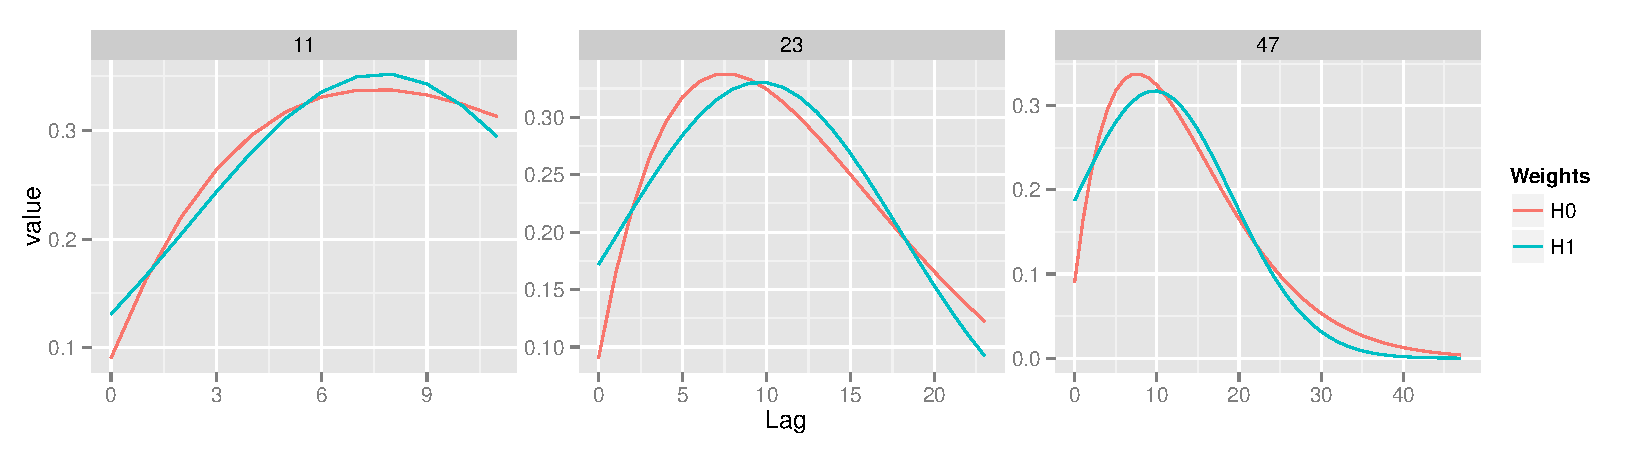
\includegraphics{Output-fig1}
\end{center}
\caption{Weights for different lags}
\label{fig:one}
\end{figure}

\begin{figure}[hb]
\begin{center}
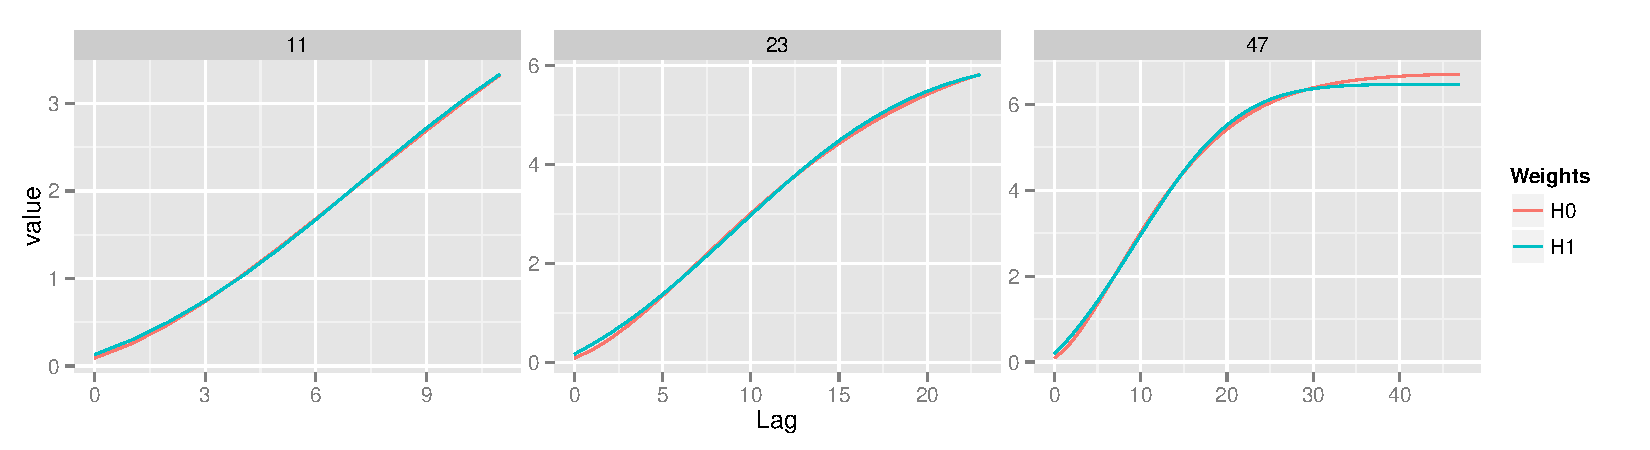
\includegraphics{Output-fig2}
\end{center}
\caption{Cumulative weights for different lags}
\label{fig:two}
\end{figure}

 
\section{Appendix}


% latex table generated in R 2.15.2 by xtable 1.7-0 package
% Fri Feb 15 12:47:04 2013
\begin{table}[ht]
\begin{center}
\caption{Empirical sizes for OLS standard errors}
\label{tab:size}
\begin{tabular}{rrrrrrrrrrrrr}
  \hline
 & $n$ & $d$ & $m$ & $\rho$ & $T_1$ & $R_{T_1}$ & $T_2$ & $R_{T_2}$ & $T_3$ & $R_{T_3}$ & $T_4$ & $R_{T_4}$ \\ 
  \hline
1 & 75 & 11 & 12 & 0.5 & 0.080 & 2000 & 0.818 & 2000 & 0.048 & 2000 & 0.447 & 2000 \\ 
  2 & 125 & 11 & 12 & 0.5 & 0.067 & 2000 & 0.782 & 2000 & 0.058 & 2000 & 0.396 & 2000 \\ 
  3 & 200 & 11 & 12 & 0.5 & 0.061 & 2000 & 0.711 & 2000 & 0.055 & 2000 & 0.328 & 2000 \\ 
  4 & 500 & 11 & 12 & 0.5 & 0.044 & 2000 & 0.566 & 2000 & 0.045 & 2000 & 0.236 & 2000 \\ 
  5 & 1000 & 11 & 12 & 0.5 & 0.054 & 2000 & 0.414 & 2000 & 0.057 & 2000 & 0.145 & 2000 \\ 
   \hline
6 & 75 & 23 & 12 & 0.5 & 0.116 & 2000 & 0.948 & 2000 & 0.064 & 2000 & 0.595 & 2000 \\ 
  7 & 125 & 23 & 12 & 0.5 & 0.085 & 2000 & 0.914 & 2000 & 0.057 & 2000 & 0.538 & 2000 \\ 
  8 & 200 & 23 & 12 & 0.5 & 0.058 & 2000 & 0.903 & 2000 & 0.048 & 2000 & 0.497 & 2000 \\ 
  9 & 500 & 23 & 12 & 0.5 & 0.060 & 2000 & 0.829 & 2000 & 0.054 & 2000 & 0.367 & 2000 \\ 
  10 & 1000 & 23 & 12 & 0.5 & 0.055 & 2000 & 0.782 & 2000 & 0.056 & 2000 & 0.285 & 2000 \\ 
   \hline
11 & 75 & 11 & 24 & 0.5 & 0.075 & 2000 & 0.799 & 2000 & 0.059 & 2000 & 0.434 & 2000 \\ 
  12 & 125 & 11 & 24 & 0.5 & 0.066 & 2000 & 0.769 & 2000 & 0.046 & 2000 & 0.405 & 2000 \\ 
  13 & 200 & 11 & 24 & 0.5 & 0.053 & 2000 & 0.718 & 2000 & 0.048 & 2000 & 0.342 & 2000 \\ 
  14 & 500 & 11 & 24 & 0.5 & 0.056 & 2000 & 0.568 & 2000 & 0.050 & 2000 & 0.216 & 2000 \\ 
  15 & 1000 & 11 & 24 & 0.5 & 0.044 & 2000 & 0.428 & 2000 & 0.048 & 2000 & 0.150 & 2000 \\ 
   \hline
16 & 75 & 23 & 24 & 0.5 & 0.115 & 2000 & 0.927 & 2000 & 0.051 & 2000 & 0.596 & 2000 \\ 
  17 & 125 & 23 & 24 & 0.5 & 0.073 & 2000 & 0.895 & 2000 & 0.049 & 2000 & 0.519 & 2000 \\ 
  18 & 200 & 23 & 24 & 0.5 & 0.063 & 2000 & 0.858 & 2000 & 0.059 & 2000 & 0.468 & 2000 \\ 
  19 & 500 & 23 & 24 & 0.5 & 0.051 & 2000 & 0.769 & 2000 & 0.044 & 2000 & 0.325 & 2000 \\ 
  20 & 1000 & 23 & 24 & 0.5 & 0.049 & 2000 & 0.678 & 2000 & 0.059 & 2000 & 0.246 & 2000 \\ 
   \hline
21 & 75 & 47 & 24 & 0.5 & 0.251 & 2000 & 0.969 & 2000 & 0.065 & 2000 & 0.750 & 2000 \\ 
  22 & 125 & 47 & 24 & 0.5 & 0.120 & 2000 & 0.971 & 2000 & 0.059 & 2000 & 0.713 & 2000 \\ 
  23 & 200 & 47 & 24 & 0.5 & 0.085 & 2000 & 0.949 & 2000 & 0.046 & 2000 & 0.649 & 2000 \\ 
  24 & 500 & 47 & 24 & 0.5 & 0.056 & 2000 & 0.917 & 2000 & 0.048 & 2000 & 0.557 & 2000 \\ 
  25 & 1000 & 47 & 24 & 0.5 & 0.052 & 2000 & 0.904 & 1999 & 0.058 & 2000 & 0.472 & 2000 \\ 
   \hline
26 & 75 & 11 & 12 & 0.9 & 0.070 & 2000 & 0.949 & 1993 & 0.058 & 2000 & 0.747 & 1986 \\ 
  27 & 125 & 11 & 12 & 0.9 & 0.059 & 2000 & 0.925 & 2000 & 0.055 & 2000 & 0.664 & 1998 \\ 
  28 & 200 & 11 & 12 & 0.9 & 0.059 & 2000 & 0.908 & 2000 & 0.049 & 2000 & 0.617 & 2000 \\ 
  29 & 500 & 11 & 12 & 0.9 & 0.050 & 2000 & 0.854 & 1995 & 0.048 & 2000 & 0.527 & 1999 \\ 
  30 & 1000 & 11 & 12 & 0.9 & 0.046 & 2000 & 0.787 & 2000 & 0.053 & 1999 & 0.425 & 2000 \\ 
   \hline
31 & 75 & 23 & 12 & 0.9 & 0.112 & 2000 & 0.986 & 1996 & 0.063 & 2000 & 0.826 & 1999 \\ 
  32 & 125 & 23 & 12 & 0.9 & 0.088 & 2000 & 0.978 & 1992 & 0.058 & 2000 & 0.794 & 1997 \\ 
  33 & 200 & 23 & 12 & 0.9 & 0.059 & 2000 & 0.968 & 1996 & 0.048 & 2000 & 0.783 & 1997 \\ 
  34 & 500 & 23 & 12 & 0.9 & 0.059 & 2000 & 0.961 & 1998 & 0.052 & 2000 & 0.684 & 1998 \\ 
  35 & 1000 & 23 & 12 & 0.9 & 0.051 & 2000 & 0.939 & 1984 & 0.051 & 2000 & 0.622 & 1984 \\ 
   \hline
36 & 75 & 11 & 24 & 0.9 & 0.080 & 2000 & 0.933 & 2000 & 0.058 & 2000 & 0.689 & 1996 \\ 
  37 & 125 & 11 & 24 & 0.9 & 0.060 & 2000 & 0.898 & 1999 & 0.054 & 2000 & 0.625 & 1999 \\ 
  38 & 200 & 11 & 24 & 0.9 & 0.052 & 2000 & 0.891 & 2000 & 0.056 & 2000 & 0.565 & 2000 \\ 
  39 & 500 & 11 & 24 & 0.9 & 0.066 & 2000 & 0.809 & 1997 & 0.057 & 2000 & 0.464 & 2000 \\ 
  40 & 1000 & 11 & 24 & 0.9 & 0.048 & 2000 & 0.738 & 2000 & 0.047 & 2000 & 0.387 & 2000 \\ 
   \hline
41 & 75 & 23 & 24 & 0.9 & 0.121 & 2000 & 0.979 & 1999 & 0.059 & 2000 & 0.834 & 1998 \\ 
  42 & 125 & 23 & 24 & 0.9 & 0.081 & 2000 & 0.966 & 1997 & 0.047 & 2000 & 0.789 & 1999 \\ 
  43 & 200 & 23 & 24 & 0.9 & 0.074 & 2000 & 0.958 & 1998 & 0.049 & 2000 & 0.759 & 1999 \\ 
  44 & 500 & 23 & 24 & 0.9 & 0.056 & 2000 & 0.935 & 2000 & 0.050 & 2000 & 0.685 & 2000 \\ 
  45 & 1000 & 23 & 24 & 0.9 & 0.053 & 2000 & 0.908 & 1995 & 0.052 & 2000 & 0.587 & 1988 \\ 
   \hline
46 & 75 & 47 & 24 & 0.9 & 0.252 & 2000 & 0.994 & 1996 & 0.062 & 2000 & 0.923 & 1997 \\ 
  47 & 125 & 47 & 24 & 0.9 & 0.125 & 2000 & 0.992 & 1985 & 0.065 & 2000 & 0.911 & 1980 \\ 
  48 & 200 & 47 & 24 & 0.9 & 0.082 & 1999 & 0.989 & 1885 & 0.051 & 1999 & 0.897 & 1882 \\ 
  49 & 500 & 47 & 24 & 0.9 & 0.057 & 2000 & 0.981 & 1963 & 0.051 & 2000 & 0.847 & 1983 \\ 
  50 & 1000 & 47 & 24 & 0.9 & 0.065 & 1996 & 0.964 & 1677 & 0.045 & 1992 & 0.778 & 1721 \\ 
   \hline
\end{tabular}
\end{center}
\end{table}
% latex table generated in R 2.15.2 by xtable 1.7-0 package
% Fri Feb 15 12:47:04 2013
\begin{table}[ht]
\begin{center}
\caption{Empirical sizes for NLS standard errors}
\label{tab:sizenls}
\begin{tabular}{rrrrrrrrrrrrr}
  \hline
 & $n$ & $d$ & $m$ & $\rho$ & $T_1'$ & $R_{T_1'}$ & $T_2'$ & $R_{T_2'}$ & $T_3'$ & $R_{T_3'}$ & $T_4'$ & $R_{T_4'}$ \\ 
  \hline
1 & 75 & 11 & 12 & 0.5 & 0.041 & 2000 & 0.035 & 2000 & 0.047 & 2000 & 0.067 & 2000 \\ 
  2 & 125 & 11 & 12 & 0.5 & 0.051 & 2000 & 0.041 & 2000 & 0.058 & 2000 & 0.068 & 2000 \\ 
  3 & 200 & 11 & 12 & 0.5 & 0.050 & 2000 & 0.041 & 2000 & 0.054 & 2000 & 0.070 & 2000 \\ 
  4 & 500 & 11 & 12 & 0.5 & 0.040 & 2000 & 0.044 & 2000 & 0.045 & 2000 & 0.059 & 2000 \\ 
  5 & 1000 & 11 & 12 & 0.5 & 0.051 & 2000 & 0.049 & 2000 & 0.058 & 2000 & 0.051 & 2000 \\ 
   \hline
6 & 75 & 23 & 12 & 0.5 & 0.033 & 2000 & 0.051 & 2000 & 0.060 & 2000 & 0.035 & 2000 \\ 
  7 & 125 & 23 & 12 & 0.5 & 0.046 & 2000 & 0.072 & 2000 & 0.057 & 2000 & 0.029 & 2000 \\ 
  8 & 200 & 23 & 12 & 0.5 & 0.039 & 2000 & 0.082 & 2000 & 0.048 & 2000 & 0.034 & 2000 \\ 
  9 & 500 & 23 & 12 & 0.5 & 0.051 & 2000 & 0.090 & 2000 & 0.055 & 2000 & 0.028 & 2000 \\ 
  10 & 1000 & 23 & 12 & 0.5 & 0.051 & 2000 & 0.089 & 2000 & 0.056 & 2000 & 0.036 & 2000 \\ 
   \hline
11 & 75 & 11 & 24 & 0.5 & 0.043 & 2000 & 0.038 & 2000 & 0.062 & 2000 & 0.054 & 2000 \\ 
  12 & 125 & 11 & 24 & 0.5 & 0.047 & 2000 & 0.036 & 2000 & 0.045 & 2000 & 0.052 & 2000 \\ 
  13 & 200 & 11 & 24 & 0.5 & 0.041 & 2000 & 0.044 & 2000 & 0.050 & 2000 & 0.062 & 2000 \\ 
  14 & 500 & 11 & 24 & 0.5 & 0.052 & 2000 & 0.051 & 2000 & 0.052 & 2000 & 0.064 & 2000 \\ 
  15 & 1000 & 11 & 24 & 0.5 & 0.042 & 2000 & 0.051 & 2000 & 0.048 & 2000 & 0.049 & 2000 \\ 
   \hline
16 & 75 & 23 & 24 & 0.5 & 0.030 & 2000 & 0.022 & 2000 & 0.052 & 2000 & 0.059 & 2000 \\ 
  17 & 125 & 23 & 24 & 0.5 & 0.035 & 2000 & 0.032 & 2000 & 0.051 & 2000 & 0.062 & 2000 \\ 
  18 & 200 & 23 & 24 & 0.5 & 0.043 & 2000 & 0.043 & 2000 & 0.057 & 2000 & 0.060 & 2000 \\ 
  19 & 500 & 23 & 24 & 0.5 & 0.041 & 2000 & 0.051 & 2000 & 0.044 & 2000 & 0.056 & 2000 \\ 
  20 & 1000 & 23 & 24 & 0.5 & 0.041 & 2000 & 0.043 & 2000 & 0.060 & 2000 & 0.058 & 2000 \\ 
   \hline
21 & 75 & 47 & 24 & 0.5 & 0.001 & 2000 & 0.000 & 2000 & 0.058 & 2000 & 0.027 & 2000 \\ 
  22 & 125 & 47 & 24 & 0.5 & 0.020 & 2000 & 0.047 & 2000 & 0.060 & 2000 & 0.037 & 2000 \\ 
  23 & 200 & 47 & 24 & 0.5 & 0.035 & 2000 & 0.081 & 2000 & 0.045 & 2000 & 0.027 & 2000 \\ 
  24 & 500 & 47 & 24 & 0.5 & 0.041 & 2000 & 0.101 & 2000 & 0.048 & 2000 & 0.029 & 2000 \\ 
  25 & 1000 & 47 & 24 & 0.5 & 0.045 & 2000 & 0.092 & 1999 & 0.058 & 2000 & 0.041 & 2000 \\ 
   \hline
26 & 75 & 11 & 12 & 0.9 & 0.041 & 2000 & 0.034 & 1993 & 0.058 & 2000 & 0.148 & 1986 \\ 
  27 & 125 & 11 & 12 & 0.9 & 0.049 & 2000 & 0.048 & 2000 & 0.054 & 2000 & 0.113 & 1998 \\ 
  28 & 200 & 11 & 12 & 0.9 & 0.048 & 2000 & 0.056 & 2000 & 0.049 & 2000 & 0.108 & 2000 \\ 
  29 & 500 & 11 & 12 & 0.9 & 0.044 & 2000 & 0.047 & 1995 & 0.048 & 2000 & 0.094 & 1999 \\ 
  30 & 1000 & 11 & 12 & 0.9 & 0.043 & 2000 & 0.052 & 2000 & 0.053 & 1999 & 0.085 & 2000 \\ 
   \hline
31 & 75 & 23 & 12 & 0.9 & 0.030 & 2000 & 0.055 & 1996 & 0.068 & 2000 & 0.067 & 1999 \\ 
  32 & 125 & 23 & 12 & 0.9 & 0.044 & 2000 & 0.076 & 1992 & 0.057 & 2000 & 0.044 & 1997 \\ 
  33 & 200 & 23 & 12 & 0.9 & 0.037 & 2000 & 0.095 & 1996 & 0.046 & 2000 & 0.043 & 1997 \\ 
  34 & 500 & 23 & 12 & 0.9 & 0.051 & 2000 & 0.107 & 1998 & 0.053 & 2000 & 0.027 & 1998 \\ 
  35 & 1000 & 23 & 12 & 0.9 & 0.046 & 2000 & 0.108 & 1984 & 0.052 & 2000 & 0.030 & 1984 \\ 
   \hline
36 & 75 & 11 & 24 & 0.9 & 0.051 & 2000 & 0.034 & 2000 & 0.060 & 2000 & 0.100 & 1996 \\ 
  37 & 125 & 11 & 24 & 0.9 & 0.043 & 2000 & 0.041 & 1999 & 0.054 & 2000 & 0.080 & 1999 \\ 
  38 & 200 & 11 & 24 & 0.9 & 0.046 & 2000 & 0.042 & 2000 & 0.058 & 2000 & 0.061 & 2000 \\ 
  39 & 500 & 11 & 24 & 0.9 & 0.063 & 2000 & 0.055 & 1997 & 0.057 & 2000 & 0.062 & 2000 \\ 
  40 & 1000 & 11 & 24 & 0.9 & 0.046 & 2000 & 0.045 & 2000 & 0.047 & 2000 & 0.063 & 2000 \\ 
   \hline
41 & 75 & 23 & 24 & 0.9 & 0.032 & 2000 & 0.024 & 1999 & 0.057 & 2000 & 0.100 & 1998 \\ 
  42 & 125 & 23 & 24 & 0.9 & 0.041 & 2000 & 0.035 & 1997 & 0.045 & 2000 & 0.106 & 1999 \\ 
  43 & 200 & 23 & 24 & 0.9 & 0.049 & 2000 & 0.038 & 1998 & 0.050 & 2000 & 0.103 & 1999 \\ 
  44 & 500 & 23 & 24 & 0.9 & 0.047 & 2000 & 0.044 & 2000 & 0.050 & 2000 & 0.089 & 2000 \\ 
  45 & 1000 & 23 & 24 & 0.9 & 0.050 & 2000 & 0.046 & 1995 & 0.053 & 2000 & 0.082 & 1988 \\ 
   \hline
46 & 75 & 47 & 24 & 0.9 & 0.000 & 2000 & 0.001 & 1996 & 0.053 & 2000 & 0.052 & 1997 \\ 
  47 & 125 & 47 & 24 & 0.9 & 0.019 & 2000 & 0.042 & 1985 & 0.061 & 2000 & 0.030 & 1980 \\ 
  48 & 200 & 47 & 24 & 0.9 & 0.030 & 1999 & 0.081 & 1885 & 0.054 & 1999 & 0.024 & 1882 \\ 
  49 & 500 & 47 & 24 & 0.9 & 0.040 & 2000 & 0.108 & 1963 & 0.053 & 2000 & 0.021 & 1983 \\ 
  50 & 1000 & 47 & 24 & 0.9 & 0.056 & 1996 & 0.110 & 1677 & 0.046 & 1992 & 0.023 & 1721 \\ 
   \hline
\end{tabular}
\end{center}
\end{table}
% latex table generated in R 2.15.2 by xtable 1.7-0 package
% Fri Feb 15 12:47:04 2013
\begin{table}[ht]
\begin{center}
\caption{Empirical power for OLS standard errors}
\label{tab:power}
\begin{tabular}{rrrrrrrrrrrrr}
  \hline
 & $n$ & $d$ & $m$ & $\rho$ & $T_1$ & $R_{T_1}$ & $T_2$ & $R_{T_2}$ & $T_3$ & $R_{T_3}$ & $T_4$ & $R_{T_4}$ \\ 
  \hline
1 & 75 & 11 & 12 & 0.5 & 0.108 & 2000 & 0.509 & 2000 & 0.141 & 2000 & 0.248 & 2000 \\ 
  2 & 125 & 11 & 12 & 0.5 & 0.111 & 2000 & 0.431 & 2000 & 0.171 & 2000 & 0.243 & 2000 \\ 
  3 & 200 & 11 & 12 & 0.5 & 0.123 & 2000 & 0.362 & 2000 & 0.213 & 2000 & 0.272 & 2000 \\ 
  4 & 500 & 11 & 12 & 0.5 & 0.243 & 2000 & 0.369 & 2000 & 0.425 & 2000 & 0.442 & 2000 \\ 
  5 & 1000 & 11 & 12 & 0.5 & 0.479 & 2000 & 0.533 & 2000 & 0.674 & 2000 & 0.675 & 2000 \\ 
   \hline
6 & 75 & 23 & 12 & 0.5 & 0.543 & 2000 & 0.958 & 2000 & 0.734 & 2000 & 0.718 & 2000 \\ 
  7 & 125 & 23 & 12 & 0.5 & 0.784 & 2000 & 0.976 & 2000 & 0.882 & 2000 & 0.784 & 2000 \\ 
  8 & 200 & 23 & 12 & 0.5 & 0.968 & 2000 & 0.995 & 2000 & 0.979 & 2000 & 0.868 & 2000 \\ 
  9 & 500 & 23 & 12 & 0.5 & 1.000 & 2000 & 1.000 & 2000 & 1.000 & 2000 & 0.988 & 2000 \\ 
  10 & 1000 & 23 & 12 & 0.5 & 1.000 & 2000 & 1.000 & 2000 & 1.000 & 2000 & 1.000 & 2000 \\ 
   \hline
11 & 75 & 11 & 24 & 0.5 & 0.093 & 2000 & 0.484 & 2000 & 0.132 & 2000 & 0.249 & 2000 \\ 
  12 & 125 & 11 & 24 & 0.5 & 0.103 & 2000 & 0.419 & 2000 & 0.154 & 2000 & 0.244 & 2000 \\ 
  13 & 200 & 11 & 24 & 0.5 & 0.118 & 2000 & 0.372 & 2000 & 0.234 & 2000 & 0.302 & 2000 \\ 
  14 & 500 & 11 & 24 & 0.5 & 0.250 & 2000 & 0.364 & 2000 & 0.464 & 2000 & 0.477 & 2000 \\ 
  15 & 1000 & 11 & 24 & 0.5 & 0.466 & 2000 & 0.526 & 2000 & 0.676 & 2000 & 0.684 & 2000 \\ 
   \hline
16 & 75 & 23 & 24 & 0.5 & 0.538 & 2000 & 0.936 & 2000 & 0.708 & 2000 & 0.699 & 2000 \\ 
  17 & 125 & 23 & 24 & 0.5 & 0.793 & 2000 & 0.972 & 2000 & 0.895 & 2000 & 0.778 & 2000 \\ 
  18 & 200 & 23 & 24 & 0.5 & 0.958 & 2000 & 0.994 & 2000 & 0.978 & 2000 & 0.873 & 2000 \\ 
  19 & 500 & 23 & 24 & 0.5 & 1.000 & 2000 & 1.000 & 2000 & 1.000 & 2000 & 0.988 & 2000 \\ 
  20 & 1000 & 23 & 24 & 0.5 & 1.000 & 2000 & 1.000 & 2000 & 1.000 & 2000 & 1.000 & 2000 \\ 
   \hline
21 & 75 & 47 & 24 & 0.5 & 0.964 & 2000 & 0.999 & 2000 & 0.968 & 2000 & 0.829 & 2000 \\ 
  22 & 125 & 47 & 24 & 0.5 & 1.000 & 2000 & 1.000 & 1999 & 0.999 & 2000 & 0.839 & 2000 \\ 
  23 & 200 & 47 & 24 & 0.5 & 1.000 & 2000 & 1.000 & 2000 & 1.000 & 2000 & 0.872 & 2000 \\ 
  24 & 500 & 47 & 24 & 0.5 & 1.000 & 2000 & 1.000 & 2000 & 1.000 & 2000 & 0.962 & 2000 \\ 
  25 & 1000 & 47 & 24 & 0.5 & 1.000 & 2000 & 1.000 & 2000 & 1.000 & 2000 & 0.996 & 2000 \\ 
   \hline
26 & 75 & 11 & 12 & 0.9 & 0.101 & 2000 & 0.821 & 1969 & 0.197 & 2000 & 0.532 & 1970 \\ 
  27 & 125 & 11 & 12 & 0.9 & 0.117 & 2000 & 0.778 & 1999 & 0.260 & 1988 & 0.478 & 1972 \\ 
  28 & 200 & 11 & 12 & 0.9 & 0.150 & 2000 & 0.733 & 2000 & 0.384 & 2000 & 0.503 & 2000 \\ 
  29 & 500 & 11 & 12 & 0.9 & 0.320 & 2000 & 0.736 & 2000 & 0.708 & 2000 & 0.699 & 2000 \\ 
  30 & 1000 & 11 & 12 & 0.9 & 0.622 & 2000 & 0.799 & 2000 & 0.918 & 2000 & 0.888 & 2000 \\ 
   \hline
31 & 75 & 23 & 12 & 0.9 & 0.919 & 2000 & 0.999 & 1996 & 0.998 & 2000 & 0.906 & 1999 \\ 
  32 & 125 & 23 & 12 & 0.9 & 0.997 & 2000 & 1.000 & 1993 & 1.000 & 2000 & 0.914 & 1995 \\ 
  33 & 200 & 23 & 12 & 0.9 & 1.000 & 2000 & 1.000 & 2000 & 1.000 & 2000 & 0.962 & 2000 \\ 
  34 & 500 & 23 & 12 & 0.9 & 1.000 & 2000 & 1.000 & 1998 & 1.000 & 2000 & 0.996 & 2000 \\ 
  35 & 1000 & 23 & 12 & 0.9 & 1.000 & 2000 & 1.000 & 1998 & 1.000 & 2000 & 1.000 & 1996 \\ 
   \hline
36 & 75 & 11 & 24 & 0.9 & 0.106 & 2000 & 0.770 & 1988 & 0.204 & 2000 & 0.460 & 1996 \\ 
  37 & 125 & 11 & 24 & 0.9 & 0.114 & 2000 & 0.738 & 2000 & 0.274 & 1982 & 0.445 & 1979 \\ 
  38 & 200 & 11 & 24 & 0.9 & 0.140 & 2000 & 0.686 & 2000 & 0.383 & 2000 & 0.480 & 1999 \\ 
  39 & 500 & 11 & 24 & 0.9 & 0.310 & 2000 & 0.660 & 2000 & 0.691 & 2000 & 0.658 & 2000 \\ 
  40 & 1000 & 11 & 24 & 0.9 & 0.625 & 2000 & 0.761 & 2000 & 0.928 & 2000 & 0.873 & 2000 \\ 
   \hline
41 & 75 & 23 & 24 & 0.9 & 0.932 & 2000 & 0.999 & 1999 & 0.998 & 2000 & 0.895 & 2000 \\ 
  42 & 125 & 23 & 24 & 0.9 & 0.999 & 2000 & 1.000 & 1997 & 1.000 & 2000 & 0.928 & 2000 \\ 
  43 & 200 & 23 & 24 & 0.9 & 1.000 & 2000 & 1.000 & 2000 & 1.000 & 2000 & 0.938 & 1999 \\ 
  44 & 500 & 23 & 24 & 0.9 & 1.000 & 2000 & 1.000 & 2000 & 1.000 & 2000 & 0.991 & 2000 \\ 
  45 & 1000 & 23 & 24 & 0.9 & 1.000 & 2000 & 1.000 & 2000 & 1.000 & 2000 & 0.998 & 1999 \\ 
   \hline
46 & 75 & 47 & 24 & 0.9 & 1.000 & 2000 & 1.000 & 1997 & 1.000 & 2000 & 0.958 & 1994 \\ 
  47 & 125 & 47 & 24 & 0.9 & 1.000 & 2000 & 1.000 & 1975 & 1.000 & 2000 & 0.961 & 1972 \\ 
  48 & 200 & 47 & 24 & 0.9 & 1.000 & 2000 & 1.000 & 1933 & 1.000 & 1999 & 0.966 & 1962 \\ 
  49 & 500 & 47 & 24 & 0.9 & 1.000 & 2000 & 1.000 & 1941 & 1.000 & 2000 & 0.988 & 1973 \\ 
  50 & 1000 & 47 & 24 & 0.9 & 1.000 & 1997 & 1.000 & 1855 & 1.000 & 2000 & 0.998 & 1867 \\ 
   \hline
\end{tabular}
\end{center}
\end{table}
% latex table generated in R 2.15.2 by xtable 1.7-0 package
% Fri Feb 15 12:47:04 2013
\begin{table}[ht]
\begin{center}
\caption{Empirical power for NLS standard errors}
\label{tab:powernls}
\begin{tabular}{rrrrrrrrrrrrr}
  \hline
 & $n$ & $d$ & $m$ & $\rho$ & $T_1'$ & $R_{T_1'}$ & $T_2'$ & $R_{T_2'}$ & $T_3'$ & $R_{T_3'}$ & $T_4'$ & $R_{T_4'}$ \\ 
  \hline
1 & 75 & 11 & 12 & 0.5 & 0.061 & 2000 & 0.049 & 2000 & 0.142 & 2000 & 0.129 & 2000 \\ 
  2 & 125 & 11 & 12 & 0.5 & 0.081 & 2000 & 0.067 & 2000 & 0.172 & 2000 & 0.153 & 2000 \\ 
  3 & 200 & 11 & 12 & 0.5 & 0.109 & 2000 & 0.089 & 2000 & 0.214 & 2000 & 0.195 & 2000 \\ 
  4 & 500 & 11 & 12 & 0.5 & 0.230 & 2000 & 0.203 & 2000 & 0.423 & 2000 & 0.388 & 2000 \\ 
  5 & 1000 & 11 & 12 & 0.5 & 0.474 & 2000 & 0.439 & 2000 & 0.673 & 2000 & 0.648 & 2000 \\ 
   \hline
6 & 75 & 23 & 12 & 0.5 & 0.292 & 2000 & 0.083 & 2000 & 0.693 & 2000 & 0.231 & 2000 \\ 
  7 & 125 & 23 & 12 & 0.5 & 0.658 & 2000 & 0.197 & 2000 & 0.860 & 2000 & 0.374 & 2000 \\ 
  8 & 200 & 23 & 12 & 0.5 & 0.955 & 2000 & 0.367 & 2000 & 0.973 & 2000 & 0.544 & 2000 \\ 
  9 & 500 & 23 & 12 & 0.5 & 1.000 & 2000 & 0.785 & 2000 & 1.000 & 2000 & 0.880 & 2000 \\ 
  10 & 1000 & 23 & 12 & 0.5 & 1.000 & 2000 & 0.980 & 2000 & 1.000 & 2000 & 0.989 & 2000 \\ 
   \hline
11 & 75 & 11 & 24 & 0.5 & 0.057 & 2000 & 0.044 & 2000 & 0.134 & 2000 & 0.121 & 2000 \\ 
  12 & 125 & 11 & 24 & 0.5 & 0.078 & 2000 & 0.059 & 2000 & 0.154 & 2000 & 0.147 & 2000 \\ 
  13 & 200 & 11 & 24 & 0.5 & 0.104 & 2000 & 0.078 & 2000 & 0.232 & 2000 & 0.217 & 2000 \\ 
  14 & 500 & 11 & 24 & 0.5 & 0.237 & 2000 & 0.200 & 2000 & 0.463 & 2000 & 0.426 & 2000 \\ 
  15 & 1000 & 11 & 24 & 0.5 & 0.461 & 2000 & 0.417 & 2000 & 0.675 & 2000 & 0.653 & 2000 \\ 
   \hline
16 & 75 & 23 & 24 & 0.5 & 0.278 & 2000 & 0.055 & 2000 & 0.668 & 2000 & 0.282 & 2000 \\ 
  17 & 125 & 23 & 24 & 0.5 & 0.681 & 2000 & 0.197 & 2000 & 0.871 & 2000 & 0.439 & 2000 \\ 
  18 & 200 & 23 & 24 & 0.5 & 0.942 & 2000 & 0.414 & 2000 & 0.969 & 2000 & 0.619 & 2000 \\ 
  19 & 500 & 23 & 24 & 0.5 & 1.000 & 2000 & 0.874 & 2000 & 1.000 & 2000 & 0.936 & 2000 \\ 
  20 & 1000 & 23 & 24 & 0.5 & 1.000 & 2000 & 0.993 & 2000 & 1.000 & 2000 & 0.999 & 2000 \\ 
   \hline
21 & 75 & 47 & 24 & 0.5 & 0.115 & 2000 & 0.003 & 2000 & 0.913 & 2000 & 0.277 & 2000 \\ 
  22 & 125 & 47 & 24 & 0.5 & 0.996 & 2000 & 0.180 & 1999 & 0.987 & 2000 & 0.387 & 2000 \\ 
  23 & 200 & 47 & 24 & 0.5 & 1.000 & 2000 & 0.353 & 2000 & 1.000 & 2000 & 0.478 & 2000 \\ 
  24 & 500 & 47 & 24 & 0.5 & 1.000 & 2000 & 0.730 & 2000 & 1.000 & 2000 & 0.717 & 2000 \\ 
  25 & 1000 & 47 & 24 & 0.5 & 1.000 & 2000 & 0.951 & 2000 & 1.000 & 2000 & 0.934 & 2000 \\ 
   \hline
26 & 75 & 11 & 12 & 0.9 & 0.058 & 2000 & 0.044 & 1969 & 0.198 & 2000 & 0.254 & 1970 \\ 
  27 & 125 & 11 & 12 & 0.9 & 0.091 & 2000 & 0.064 & 1999 & 0.260 & 1988 & 0.217 & 1972 \\ 
  28 & 200 & 11 & 12 & 0.9 & 0.130 & 2000 & 0.093 & 2000 & 0.384 & 2000 & 0.276 & 2000 \\ 
  29 & 500 & 11 & 12 & 0.9 & 0.311 & 2000 & 0.195 & 2000 & 0.708 & 2000 & 0.517 & 2000 \\ 
  30 & 1000 & 11 & 12 & 0.9 & 0.615 & 2000 & 0.425 & 2000 & 0.918 & 2000 & 0.804 & 2000 \\ 
   \hline
31 & 75 & 23 & 12 & 0.9 & 0.747 & 2000 & 0.085 & 1996 & 0.998 & 2000 & 0.251 & 1999 \\ 
  32 & 125 & 23 & 12 & 0.9 & 0.992 & 2000 & 0.161 & 1993 & 1.000 & 2000 & 0.365 & 1995 \\ 
  33 & 200 & 23 & 12 & 0.9 & 1.000 & 2000 & 0.240 & 2000 & 1.000 & 2000 & 0.502 & 2000 \\ 
  34 & 500 & 23 & 12 & 0.9 & 1.000 & 2000 & 0.538 & 1998 & 1.000 & 2000 & 0.877 & 2000 \\ 
  35 & 1000 & 23 & 12 & 0.9 & 1.000 & 2000 & 0.788 & 1998 & 1.000 & 2000 & 0.989 & 1996 \\ 
   \hline
36 & 75 & 11 & 24 & 0.9 & 0.070 & 2000 & 0.041 & 1988 & 0.203 & 2000 & 0.190 & 1996 \\ 
  37 & 125 & 11 & 24 & 0.9 & 0.088 & 2000 & 0.050 & 2000 & 0.276 & 1982 & 0.186 & 1979 \\ 
  38 & 200 & 11 & 24 & 0.9 & 0.119 & 2000 & 0.073 & 2000 & 0.384 & 2000 & 0.231 & 1999 \\ 
  39 & 500 & 11 & 24 & 0.9 & 0.302 & 2000 & 0.186 & 2000 & 0.689 & 2000 & 0.509 & 2000 \\ 
  40 & 1000 & 11 & 24 & 0.9 & 0.618 & 2000 & 0.397 & 2000 & 0.928 & 2000 & 0.784 & 2000 \\ 
   \hline
41 & 75 & 23 & 24 & 0.9 & 0.774 & 2000 & 0.067 & 1999 & 0.996 & 2000 & 0.322 & 2000 \\ 
  42 & 125 & 23 & 24 & 0.9 & 0.994 & 2000 & 0.150 & 1997 & 1.000 & 2000 & 0.451 & 2000 \\ 
  43 & 200 & 23 & 24 & 0.9 & 1.000 & 2000 & 0.272 & 2000 & 1.000 & 2000 & 0.572 & 1999 \\ 
  44 & 500 & 23 & 24 & 0.9 & 1.000 & 2000 & 0.625 & 2000 & 1.000 & 2000 & 0.871 & 2000 \\ 
  45 & 1000 & 23 & 24 & 0.9 & 1.000 & 2000 & 0.897 & 2000 & 1.000 & 2000 & 0.989 & 1999 \\ 
   \hline
46 & 75 & 47 & 24 & 0.9 & 0.989 & 2000 & 0.014 & 1997 & 1.000 & 2000 & 0.289 & 1994 \\ 
  47 & 125 & 47 & 24 & 0.9 & 1.000 & 2000 & 0.125 & 1975 & 1.000 & 2000 & 0.376 & 1972 \\ 
  48 & 200 & 47 & 24 & 0.9 & 1.000 & 2000 & 0.246 & 1933 & 1.000 & 1999 & 0.501 & 1962 \\ 
  49 & 500 & 47 & 24 & 0.9 & 1.000 & 2000 & 0.535 & 1941 & 1.000 & 2000 & 0.700 & 1973 \\ 
  50 & 1000 & 47 & 24 & 0.9 & 1.000 & 1997 & 0.818 & 1855 & 1.000 & 2000 & 0.919 & 1867 \\ 
   \hline
\end{tabular}
\end{center}
\end{table}
% latex table generated in R 2.15.2 by xtable 1.7-0 package
% Fri Feb 15 12:47:04 2013
\begin{table}[ht]
\begin{center}
\caption{Adjusted empirical power for OLS standard errors}
\label{tab:adjpower}
\begin{tabular}{rrrrrrrrrrrrr}
  \hline
 & $n$ & $d$ & $m$ & $\rho$ & $T_1$ & $R_{T_1}$ & $T_2$ & $R_{T_2}$ & $T_3$ & $R_{T_3}$ & $T_4$ & $R_{T_4}$ \\ 
  \hline
1 & 75 & 11 & 12 & 0.5 & 0.070 & 2000 & 0.000 & 2000 & 0.143 & 2000 & 0.003 & 2000 \\ 
  2 & 125 & 11 & 12 & 0.5 & 0.081 & 2000 & 0.000 & 2000 & 0.162 & 2000 & 0.002 & 2000 \\ 
  3 & 200 & 11 & 12 & 0.5 & 0.107 & 2000 & 0.000 & 2000 & 0.203 & 2000 & 0.004 & 2000 \\ 
  4 & 500 & 11 & 12 & 0.5 & 0.265 & 2000 & 0.000 & 2000 & 0.441 & 2000 & 0.038 & 2000 \\ 
  5 & 1000 & 11 & 12 & 0.5 & 0.472 & 2000 & 0.001 & 2000 & 0.664 & 2000 & 0.418 & 2000 \\ 
   \hline
6 & 75 & 23 & 12 & 0.5 & 0.385 & 2000 & 0.000 & 2000 & 0.704 & 2000 & 0.035 & 2000 \\ 
  7 & 125 & 23 & 12 & 0.5 & 0.670 & 2000 & 0.003 & 2000 & 0.874 & 2000 & 0.045 & 2000 \\ 
  8 & 200 & 23 & 12 & 0.5 & 0.965 & 2000 & 0.002 & 2000 & 0.979 & 2000 & 0.082 & 2000 \\ 
  9 & 500 & 23 & 12 & 0.5 & 1.000 & 2000 & 0.011 & 2000 & 1.000 & 2000 & 0.627 & 2000 \\ 
  10 & 1000 & 23 & 12 & 0.5 & 1.000 & 2000 & 0.024 & 2000 & 1.000 & 2000 & 0.995 & 2000 \\ 
   \hline
11 & 75 & 11 & 24 & 0.5 & 0.070 & 2000 & 0.000 & 2000 & 0.129 & 2000 & 0.004 & 2000 \\ 
  12 & 125 & 11 & 24 & 0.5 & 0.084 & 2000 & 0.000 & 2000 & 0.167 & 2000 & 0.003 & 2000 \\ 
  13 & 200 & 11 & 24 & 0.5 & 0.116 & 2000 & 0.000 & 2000 & 0.236 & 2000 & 0.007 & 2000 \\ 
  14 & 500 & 11 & 24 & 0.5 & 0.234 & 2000 & 0.000 & 2000 & 0.464 & 2000 & 0.067 & 2000 \\ 
  15 & 1000 & 11 & 24 & 0.5 & 0.469 & 2000 & 0.000 & 2000 & 0.682 & 2000 & 0.382 & 2000 \\ 
   \hline
16 & 75 & 23 & 24 & 0.5 & 0.368 & 2000 & 0.004 & 2000 & 0.707 & 2000 & 0.035 & 2000 \\ 
  17 & 125 & 23 & 24 & 0.5 & 0.741 & 2000 & 0.004 & 2000 & 0.897 & 2000 & 0.035 & 2000 \\ 
  18 & 200 & 23 & 24 & 0.5 & 0.952 & 2000 & 0.004 & 2000 & 0.973 & 2000 & 0.091 & 2000 \\ 
  19 & 500 & 23 & 24 & 0.5 & 1.000 & 2000 & 0.009 & 2000 & 1.000 & 2000 & 0.859 & 2000 \\ 
  20 & 1000 & 23 & 24 & 0.5 & 1.000 & 2000 & 0.103 & 2000 & 1.000 & 2000 & 0.999 & 2000 \\ 
   \hline
21 & 75 & 47 & 24 & 0.5 & 0.764 & 2000 & 0.020 & 2000 & 0.961 & 2000 & 0.102 & 2000 \\ 
  22 & 125 & 47 & 24 & 0.5 & 0.999 & 2000 & 0.013 & 1999 & 0.998 & 2000 & 0.080 & 2000 \\ 
  23 & 200 & 47 & 24 & 0.5 & 1.000 & 2000 & 0.022 & 2000 & 1.000 & 2000 & 0.158 & 2000 \\ 
  24 & 500 & 47 & 24 & 0.5 & 1.000 & 2000 & 0.031 & 2000 & 1.000 & 2000 & 0.516 & 2000 \\ 
  25 & 1000 & 47 & 24 & 0.5 & 1.000 & 2000 & 0.062 & 2000 & 1.000 & 2000 & 0.958 & 2000 \\ 
   \hline
26 & 75 & 11 & 12 & 0.9 & 0.074 & 2000 & 0.000 & 1969 & 0.181 & 2000 & 0.016 & 1970 \\ 
  27 & 125 & 11 & 12 & 0.9 & 0.092 & 2000 & 0.000 & 1999 & 0.253 & 1988 & 0.025 & 1972 \\ 
  28 & 200 & 11 & 12 & 0.9 & 0.135 & 2000 & 0.000 & 2000 & 0.389 & 2000 & 0.039 & 2000 \\ 
  29 & 500 & 11 & 12 & 0.9 & 0.312 & 2000 & 0.000 & 2000 & 0.712 & 2000 & 0.007 & 2000 \\ 
  30 & 1000 & 11 & 12 & 0.9 & 0.626 & 2000 & 0.000 & 2000 & 0.920 & 2000 & 0.048 & 2000 \\ 
   \hline
31 & 75 & 23 & 12 & 0.9 & 0.828 & 2000 & 0.006 & 1996 & 0.998 & 2000 & 0.063 & 1999 \\ 
  32 & 125 & 23 & 12 & 0.9 & 0.992 & 2000 & 0.007 & 1993 & 1.000 & 2000 & 0.061 & 1995 \\ 
  33 & 200 & 23 & 12 & 0.9 & 1.000 & 2000 & 0.005 & 2000 & 1.000 & 2000 & 0.059 & 2000 \\ 
  34 & 500 & 23 & 12 & 0.9 & 1.000 & 2000 & 0.004 & 1998 & 1.000 & 2000 & 0.078 & 2000 \\ 
  35 & 1000 & 23 & 12 & 0.9 & 1.000 & 2000 & 0.015 & 1998 & 1.000 & 2000 & 0.541 & 1996 \\ 
   \hline
36 & 75 & 11 & 24 & 0.9 & 0.070 & 2000 & 0.000 & 1988 & 0.195 & 2000 & 0.038 & 1996 \\ 
  37 & 125 & 11 & 24 & 0.9 & 0.098 & 2000 & 0.000 & 2000 & 0.264 & 1982 & 0.030 & 1979 \\ 
  38 & 200 & 11 & 24 & 0.9 & 0.124 & 2000 & 0.000 & 2000 & 0.359 & 2000 & 0.018 & 1999 \\ 
  39 & 500 & 11 & 24 & 0.9 & 0.260 & 2000 & 0.000 & 2000 & 0.673 & 2000 & 0.007 & 2000 \\ 
  40 & 1000 & 11 & 24 & 0.9 & 0.631 & 2000 & 0.001 & 2000 & 0.935 & 2000 & 0.086 & 2000 \\ 
   \hline
41 & 75 & 23 & 24 & 0.9 & 0.820 & 2000 & 0.005 & 1999 & 0.998 & 2000 & 0.051 & 2000 \\ 
  42 & 125 & 23 & 24 & 0.9 & 0.997 & 2000 & 0.009 & 1997 & 1.000 & 2000 & 0.050 & 2000 \\ 
  43 & 200 & 23 & 24 & 0.9 & 1.000 & 2000 & 0.003 & 2000 & 1.000 & 2000 & 0.050 & 1999 \\ 
  44 & 500 & 23 & 24 & 0.9 & 1.000 & 2000 & 0.009 & 2000 & 1.000 & 2000 & 0.111 & 2000 \\ 
  45 & 1000 & 23 & 24 & 0.9 & 1.000 & 2000 & 0.015 & 2000 & 1.000 & 2000 & 0.954 & 1999 \\ 
   \hline
46 & 75 & 47 & 24 & 0.9 & 1.000 & 2000 & 0.021 & 1997 & 1.000 & 2000 & 0.070 & 1994 \\ 
  47 & 125 & 47 & 24 & 0.9 & 1.000 & 2000 & 0.014 & 1975 & 1.000 & 2000 & 0.059 & 1972 \\ 
  48 & 200 & 47 & 24 & 0.9 & 1.000 & 2000 & 0.011 & 1933 & 1.000 & 1999 & 0.099 & 1962 \\ 
  49 & 500 & 47 & 24 & 0.9 & 1.000 & 2000 & 0.060 & 1941 & 1.000 & 2000 & 0.511 & 1973 \\ 
  50 & 1000 & 47 & 24 & 0.9 & 1.000 & 1997 & 0.035 & 1855 & 1.000 & 2000 & 0.859 & 1867 \\ 
   \hline
\end{tabular}
\end{center}
\end{table}
% latex table generated in R 2.15.2 by xtable 1.7-0 package
% Fri Feb 15 12:47:04 2013
\begin{table}[ht]
\begin{center}
\caption{Adjusted empirical power for NLS standard errors}
\label{tab:adjpowernls}
\begin{tabular}{rrrrrrrrrrrrr}
  \hline
 & $n$ & $d$ & $m$ & $\rho$ & $T_1'$ & $R_{T_1'}$ & $T_2'$ & $R_{T_2'}$ & $T_3'$ & $R_{T_3'}$ & $T_4'$ & $R_{T_4'}$ \\ 
  \hline
1 & 75 & 11 & 12 & 0.5 & 0.070 & 2000 & 0.067 & 2000 & 0.146 & 2000 & 0.106 & 2000 \\ 
  2 & 125 & 11 & 12 & 0.5 & 0.081 & 2000 & 0.083 & 2000 & 0.161 & 2000 & 0.125 & 2000 \\ 
  3 & 200 & 11 & 12 & 0.5 & 0.107 & 2000 & 0.097 & 2000 & 0.203 & 2000 & 0.170 & 2000 \\ 
  4 & 500 & 11 & 12 & 0.5 & 0.265 & 2000 & 0.210 & 2000 & 0.441 & 2000 & 0.356 & 2000 \\ 
  5 & 1000 & 11 & 12 & 0.5 & 0.472 & 2000 & 0.440 & 2000 & 0.663 & 2000 & 0.650 & 2000 \\ 
   \hline
6 & 75 & 23 & 12 & 0.5 & 0.385 & 2000 & 0.079 & 2000 & 0.657 & 2000 & 0.286 & 2000 \\ 
  7 & 125 & 23 & 12 & 0.5 & 0.670 & 2000 & 0.159 & 2000 & 0.843 & 2000 & 0.427 & 2000 \\ 
  8 & 200 & 23 & 12 & 0.5 & 0.965 & 2000 & 0.276 & 2000 & 0.975 & 2000 & 0.597 & 2000 \\ 
  9 & 500 & 23 & 12 & 0.5 & 1.000 & 2000 & 0.725 & 2000 & 1.000 & 2000 & 0.905 & 2000 \\ 
  10 & 1000 & 23 & 12 & 0.5 & 1.000 & 2000 & 0.970 & 2000 & 1.000 & 2000 & 0.992 & 2000 \\ 
   \hline
11 & 75 & 11 & 24 & 0.5 & 0.070 & 2000 & 0.052 & 2000 & 0.126 & 2000 & 0.113 & 2000 \\ 
  12 & 125 & 11 & 24 & 0.5 & 0.084 & 2000 & 0.079 & 2000 & 0.171 & 2000 & 0.144 & 2000 \\ 
  13 & 200 & 11 & 24 & 0.5 & 0.116 & 2000 & 0.088 & 2000 & 0.233 & 2000 & 0.189 & 2000 \\ 
  14 & 500 & 11 & 24 & 0.5 & 0.234 & 2000 & 0.195 & 2000 & 0.460 & 2000 & 0.394 & 2000 \\ 
  15 & 1000 & 11 & 24 & 0.5 & 0.469 & 2000 & 0.411 & 2000 & 0.681 & 2000 & 0.655 & 2000 \\ 
   \hline
16 & 75 & 23 & 24 & 0.5 & 0.368 & 2000 & 0.106 & 2000 & 0.665 & 2000 & 0.273 & 2000 \\ 
  17 & 125 & 23 & 24 & 0.5 & 0.741 & 2000 & 0.245 & 2000 & 0.867 & 2000 & 0.413 & 2000 \\ 
  18 & 200 & 23 & 24 & 0.5 & 0.952 & 2000 & 0.426 & 2000 & 0.964 & 2000 & 0.605 & 2000 \\ 
  19 & 500 & 23 & 24 & 0.5 & 1.000 & 2000 & 0.871 & 2000 & 1.000 & 2000 & 0.936 & 2000 \\ 
  20 & 1000 & 23 & 24 & 0.5 & 1.000 & 2000 & 0.993 & 2000 & 1.000 & 2000 & 0.998 & 2000 \\ 
   \hline
21 & 75 & 47 & 24 & 0.5 & 0.764 & 2000 & 0.113 & 2000 & 0.900 & 2000 & 0.325 & 2000 \\ 
  22 & 125 & 47 & 24 & 0.5 & 0.999 & 2000 & 0.184 & 1999 & 0.985 & 2000 & 0.409 & 2000 \\ 
  23 & 200 & 47 & 24 & 0.5 & 1.000 & 2000 & 0.323 & 2000 & 1.000 & 2000 & 0.508 & 2000 \\ 
  24 & 500 & 47 & 24 & 0.5 & 1.000 & 2000 & 0.676 & 2000 & 1.000 & 2000 & 0.741 & 2000 \\ 
  25 & 1000 & 47 & 24 & 0.5 & 1.000 & 2000 & 0.935 & 2000 & 1.000 & 2000 & 0.941 & 2000 \\ 
   \hline
26 & 75 & 11 & 12 & 0.9 & 0.074 & 2000 & 0.057 & 1969 & 0.173 & 2000 & 0.173 & 1970 \\ 
  27 & 125 & 11 & 12 & 0.9 & 0.092 & 2000 & 0.070 & 1999 & 0.249 & 1988 & 0.125 & 1972 \\ 
  28 & 200 & 11 & 12 & 0.9 & 0.135 & 2000 & 0.084 & 2000 & 0.386 & 2000 & 0.158 & 2000 \\ 
  29 & 500 & 11 & 12 & 0.9 & 0.312 & 2000 & 0.219 & 2000 & 0.713 & 2000 & 0.426 & 2000 \\ 
  30 & 1000 & 11 & 12 & 0.9 & 0.626 & 2000 & 0.413 & 2000 & 0.919 & 2000 & 0.799 & 2000 \\ 
   \hline
31 & 75 & 23 & 12 & 0.9 & 0.828 & 2000 & 0.076 & 1996 & 0.997 & 2000 & 0.292 & 1999 \\ 
  32 & 125 & 23 & 12 & 0.9 & 0.992 & 2000 & 0.129 & 1993 & 1.000 & 2000 & 0.445 & 1995 \\ 
  33 & 200 & 23 & 12 & 0.9 & 1.000 & 2000 & 0.176 & 2000 & 1.000 & 2000 & 0.539 & 2000 \\ 
  34 & 500 & 23 & 12 & 0.9 & 1.000 & 2000 & 0.452 & 1998 & 1.000 & 2000 & 0.904 & 2000 \\ 
  35 & 1000 & 23 & 12 & 0.9 & 1.000 & 2000 & 0.703 & 1998 & 1.000 & 2000 & 0.991 & 1996 \\ 
   \hline
36 & 75 & 11 & 24 & 0.9 & 0.070 & 2000 & 0.055 & 1988 & 0.186 & 2000 & 0.148 & 1996 \\ 
  37 & 125 & 11 & 24 & 0.9 & 0.097 & 2000 & 0.054 & 2000 & 0.262 & 1982 & 0.136 & 1979 \\ 
  38 & 200 & 11 & 24 & 0.9 & 0.124 & 2000 & 0.091 & 2000 & 0.364 & 2000 & 0.204 & 1999 \\ 
  39 & 500 & 11 & 24 & 0.9 & 0.260 & 2000 & 0.165 & 2000 & 0.671 & 2000 & 0.473 & 2000 \\ 
  40 & 1000 & 11 & 24 & 0.9 & 0.631 & 2000 & 0.414 & 2000 & 0.934 & 2000 & 0.781 & 2000 \\ 
   \hline
41 & 75 & 23 & 24 & 0.9 & 0.820 & 2000 & 0.106 & 1999 & 0.996 & 2000 & 0.248 & 2000 \\ 
  42 & 125 & 23 & 24 & 0.9 & 0.997 & 2000 & 0.175 & 1997 & 1.000 & 2000 & 0.376 & 2000 \\ 
  43 & 200 & 23 & 24 & 0.9 & 1.000 & 2000 & 0.292 & 2000 & 1.000 & 2000 & 0.482 & 1999 \\ 
  44 & 500 & 23 & 24 & 0.9 & 1.000 & 2000 & 0.645 & 2000 & 1.000 & 2000 & 0.835 & 2000 \\ 
  45 & 1000 & 23 & 24 & 0.9 & 1.000 & 2000 & 0.903 & 2000 & 1.000 & 2000 & 0.982 & 1999 \\ 
   \hline
46 & 75 & 47 & 24 & 0.9 & 1.000 & 2000 & 0.090 & 1997 & 1.000 & 2000 & 0.291 & 1994 \\ 
  47 & 125 & 47 & 24 & 0.9 & 1.000 & 2000 & 0.135 & 1975 & 1.000 & 2000 & 0.408 & 1972 \\ 
  48 & 200 & 47 & 24 & 0.9 & 1.000 & 2000 & 0.213 & 1933 & 1.000 & 1999 & 0.537 & 1962 \\ 
  49 & 500 & 47 & 24 & 0.9 & 1.000 & 2000 & 0.427 & 1941 & 1.000 & 2000 & 0.754 & 1973 \\ 
  50 & 1000 & 47 & 24 & 0.9 & 1.000 & 1997 & 0.737 & 1855 & 1.000 & 2000 & 0.934 & 1867 \\ 
   \hline
\end{tabular}
\end{center}
\end{table}\end{document}

\newpage
\section{Size with different starting values and gradient threshold 15}
% latex table generated in R 2.15.2 by xtable 1.7-0 package
% Fri Feb 15 12:47:04 2013
\begin{tabular}{rrrrrrrrrrr}
  \hline
 & n & d & m & ar & nls & nnls & td & ntd & td2 & ntd2 \\ 
  \hline
1 & 75 & 11 & 12 & 0.5 & 0.079 & 2000 & 0.060 & 2000 & 0.000 & 2000 \\ 
  2 & 125 & 11 & 12 & 0.5 & 0.066 & 2000 & 0.052 & 2000 & 0.000 & 2000 \\ 
  3 & 200 & 11 & 12 & 0.5 & 0.051 & 2000 & 0.055 & 2000 & 0.000 & 2000 \\ 
  4 & 500 & 11 & 12 & 0.5 & 0.047 & 2000 & 0.050 & 2000 & 0.000 & 2000 \\ 
  5 & 1000 & 11 & 12 & 0.5 & 0.060 & 2000 & 0.049 & 2000 & 0.000 & 2000 \\ 
   \hline
6 & 75 & 23 & 12 & 0.5 & 0.117 & 2000 & 0.056 & 2000 & 0.000 & 2000 \\ 
  7 & 125 & 23 & 12 & 0.5 & 0.081 & 2000 & 0.060 & 2000 & 0.000 & 2000 \\ 
  8 & 200 & 23 & 12 & 0.5 & 0.065 & 2000 & 0.057 & 2000 & 0.000 & 2000 \\ 
  9 & 500 & 23 & 12 & 0.5 & 0.051 & 2000 & 0.052 & 2000 & 0.000 & 2000 \\ 
  10 & 1000 & 23 & 12 & 0.5 & 0.059 & 2000 & 0.061 & 2000 & 0.000 & 2000 \\ 
   \hline
11 & 75 & 11 & 24 & 0.5 & 0.073 & 2000 & 0.064 & 2000 & 0.000 & 2000 \\ 
  12 & 125 & 11 & 24 & 0.5 & 0.063 & 2000 & 0.045 & 2000 & 0.000 & 2000 \\ 
  13 & 200 & 11 & 24 & 0.5 & 0.060 & 2000 & 0.056 & 2000 & 0.000 & 2000 \\ 
  14 & 500 & 11 & 24 & 0.5 & 0.067 & 2000 & 0.046 & 2000 & 0.000 & 2000 \\ 
  15 & 1000 & 11 & 24 & 0.5 & 0.052 & 2000 & 0.056 & 2000 & 0.000 & 2000 \\ 
   \hline
16 & 75 & 23 & 24 & 0.5 & 0.117 & 2000 & 0.048 & 2000 & 0.000 & 2000 \\ 
  17 & 125 & 23 & 24 & 0.5 & 0.084 & 2000 & 0.055 & 2000 & 0.000 & 2000 \\ 
  18 & 200 & 23 & 24 & 0.5 & 0.067 & 2000 & 0.057 & 2000 & 0.000 & 2000 \\ 
  19 & 500 & 23 & 24 & 0.5 & 0.064 & 2000 & 0.043 & 2000 & 0.000 & 2000 \\ 
  20 & 1000 & 23 & 24 & 0.5 & 0.048 & 2000 & 0.056 & 2000 & 0.000 & 2000 \\ 
   \hline
21 & 75 & 47 & 24 & 0.5 & 0.260 & 2000 & 0.061 & 2000 & 0.000 & 2000 \\ 
  22 & 125 & 47 & 24 & 0.5 & 0.116 & 2000 & 0.058 & 2000 & 0.000 & 2000 \\ 
  23 & 200 & 47 & 24 & 0.5 & 0.098 & 2000 & 0.050 & 2000 & 0.000 & 1999 \\ 
  24 & 500 & 47 & 24 & 0.5 & 0.072 & 2000 & 0.049 & 2000 & 0.000 & 2000 \\ 
  25 & 1000 & 47 & 24 & 0.5 & 0.057 & 2000 & 0.051 & 1999 & 0.000 & 1999 \\ 
   \hline
26 & 75 & 11 & 12 & 0.9 & 0.085 & 2000 & 0.057 & 2000 & 0.015 & 1989 \\ 
  27 & 125 & 11 & 12 & 0.9 & 0.062 & 2000 & 0.064 & 2000 & 0.010 & 1997 \\ 
  28 & 200 & 11 & 12 & 0.9 & 0.059 & 2000 & 0.060 & 2000 & 0.003 & 2000 \\ 
  29 & 500 & 11 & 12 & 0.9 & 0.051 & 2000 & 0.051 & 2000 & 0.000 & 1997 \\ 
  30 & 1000 & 11 & 12 & 0.9 & 0.053 & 2000 & 0.049 & 2000 & 0.000 & 1999 \\ 
   \hline
31 & 75 & 23 & 12 & 0.9 & 0.117 & 2000 & 0.058 & 2000 & 0.006 & 1996 \\ 
  32 & 125 & 23 & 12 & 0.9 & 0.090 & 2000 & 0.057 & 2000 & 0.003 & 1991 \\ 
  33 & 200 & 23 & 12 & 0.9 & 0.064 & 2000 & 0.055 & 2000 & 0.000 & 1994 \\ 
  34 & 500 & 23 & 12 & 0.9 & 0.059 & 2000 & 0.053 & 2000 & 0.000 & 2000 \\ 
  35 & 1000 & 23 & 12 & 0.9 & 0.043 & 2000 & 0.054 & 1999 & 0.000 & 1992 \\ 
   \hline
36 & 75 & 11 & 24 & 0.9 & 0.076 & 2000 & 0.060 & 2000 & 0.004 & 1998 \\ 
  37 & 125 & 11 & 24 & 0.9 & 0.065 & 2000 & 0.054 & 2000 & 0.002 & 1999 \\ 
  38 & 200 & 11 & 24 & 0.9 & 0.062 & 2000 & 0.048 & 2000 & 0.000 & 2000 \\ 
  39 & 500 & 11 & 24 & 0.9 & 0.049 & 2000 & 0.052 & 2000 & 0.000 & 2000 \\ 
  40 & 1000 & 11 & 24 & 0.9 & 0.052 & 2000 & 0.049 & 2000 & 0.000 & 2000 \\ 
   \hline
41 & 75 & 23 & 24 & 0.9 & 0.106 & 2000 & 0.063 & 2000 & 0.001 & 2000 \\ 
  42 & 125 & 23 & 24 & 0.9 & 0.079 & 2000 & 0.059 & 2000 & 0.001 & 1997 \\ 
  43 & 200 & 23 & 24 & 0.9 & 0.069 & 2000 & 0.053 & 2000 & 0.000 & 1997 \\ 
  44 & 500 & 23 & 24 & 0.9 & 0.061 & 2000 & 0.048 & 2000 & 0.000 & 1999 \\ 
  45 & 1000 & 23 & 24 & 0.9 & 0.056 & 1999 & 0.050 & 1999 & 0.000 & 1995 \\ 
   \hline
46 & 75 & 47 & 24 & 0.9 & 0.253 & 2000 & 0.066 & 2000 & 0.003 & 1993 \\ 
  47 & 125 & 47 & 24 & 0.9 & 0.111 & 2000 & 0.059 & 2000 & 0.000 & 1977 \\ 
  48 & 200 & 47 & 24 & 0.9 & 0.074 & 2000 & 0.055 & 1999 & 0.001 & 1884 \\ 
  49 & 500 & 47 & 24 & 0.9 & 0.065 & 2000 & 0.049 & 2000 & 0.000 & 1986 \\ 
  50 & 1000 & 47 & 24 & 0.9 & 0.060 & 1998 & 0.050 & 1996 & 0.000 & 1706 \\ 
   \hline
\end{tabular}
\end{document}
